\section{The Dirac delta function}
\setcounter{example}{0}
\subsection{Delta Sequences}
In physics, we often consider the idea of a point mass. Suppose we have a unit point mass at \(x=0\) with mass density given by \(w(x)\). We are interested in the mass but do not know the details of its density. We do, however, know that the \(w(x)\) will be highly localized in space and that 
\begin{equation}
    \int_{-\infty}^{\infty} w(x) dx = 1,
\end{equation}
so that the net mass is unity.

We expect two highly concentrated unit mass densities to produce masses with nearly identical physical effects. As such, we might simplify the problem by deciding, a priori, on a definite form for \(w\), such as
\begin{equation}
    w_k(x) = \begin{cases}
        \frac{k}{2}, & |x|<\frac{1}{k}\\
        0, & |x|>\frac{1}{k}
    \end{cases}
\end{equation}
or
\begin{equation}
    w_k(x)=\frac{k}{\pi (1+k^2x^2)}\,,
\end{equation}
where \(k\) is some larger natural number. In Fig 3.2, we see that \(w\) becomes highly concentrated at \(x=0\) when \(k\) is large.

\begin{figure}
    \centering
    \begin{tikzpicture}
        \def \a {1}
        \def \b {2}
        \def \c {3}
        \begin{axis}[
            axis lines = middle,
            xlabel = \(x\),
            ylabel = \(w_k(x)\),
            ymin = 0,
            ymax = 4.3,
            xmin = -1,
            xmax = 1,
            x label style = {anchor=north},
            xtick = {0},
            ytick= {0},
        ] 
        \addplot [mark=none] coordinates {(1/2, 0) (1/2, 1)};
        \addplot [mark=none] coordinates {(-1/2, 0) (-1/2, 1)};
        \addplot [mark=none] coordinates {(-1/2, 1) (1/2, 1)};
        \node at (axis cs:0.62, 0.32) {$k=2$};
        \addplot [mark=none] coordinates {(1/4, 0) (1/4, 4/2)};
        \addplot [mark=none] coordinates {(-1/4, 0) (-1/4, 4/2)};
        \addplot [mark=none] coordinates {(-1/4, 4/2) (1/4, 4/2)};  
        \node at (axis cs:0.36, 1.5) {$k=4$};  
        \addplot [mark=none] coordinates {(1/8, 0) (1/8, 8/2)};
        \addplot [mark=none] coordinates {(-1/8, 0) (-1/8, 8/2)};
        \addplot [mark=none] coordinates {(-1/8, 8/2) (1/8, 8/2)};  
        \node at (axis cs:0.25, 3) {$k=8$};  
        \end{axis}
    \end{tikzpicture}
    \caption{Mass Density; eq 3.2}
\end{figure}

\begin{figure}
    \centering
    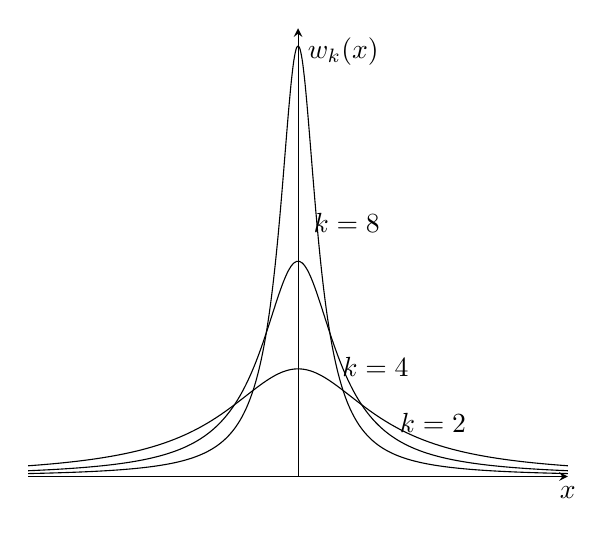
\begin{tikzpicture}
        \begin{axis}[
            axis lines = middle,
            xlabel = \(x\),
            ylabel = \(w_k(x)\),
            x label style = {anchor=north},
            xtick = {0},
            ytick= {0},
            ymin=0,
            ymax = 2.65,
            restrict y to domain=0:2.65
        ]
            \addplot[
                samples=200, 
                smooth,
                domain = -1.5:1.5
                ] 
                {2/(pi*(1+2^2*x^2))};
                \node at (axis cs:0.75, 0.32) {$k=2$};
            \addplot[
                samples=200, 
                smooth,
                domain = -1.5:1.5
                ] 
                {4/(pi*(1+4^2*x^2))};
                \node at (axis cs:0.43, 0.65) {$k=4$};
            \addplot[
                samples=200, 
                smooth,
                domain = -1.5:1.5
                ] 
                {8/(pi*(1+8^2*x^2))};
                \node at (axis cs:0.27, 1.5) {$k=8$};
        \end{axis}
    \end{tikzpicture}
    \caption{Mass Density;  eq. 3.3}
\end{figure}

If we let \(k \rightarrow \infty\), then the mass distribution approaches our idea of a point mass at \(x=0\). Calling this \(\delta(x)\), we would like to write,
\begin{equation} \label{eq:deltaSeqLim}
    \delta(x)\ "="\ \lim_{k\rightarrow \infty} w_k(x).
\end{equation}
This definition feels intuitive, but it is not a rigorous definition of the Dirac delta function because the limit is infinite for \(x=0\). That is, the right-hand side is not a function. We instead define the Dirac delta function, \(\d(x)\), in the following way
\begin{equation}
    \intR h(x)\d(x)dx = \lim_{k\rightarrow \inf}\intR h(x)w_k(x)dx
\end{equation}
and call \(w_k(x)\) a \df{\(\d\)-sequence}. This way of defining the Dirac delta function is more rigorous while still being intuitive because it is related to our understanding of delta sequences. However, keep in mind that the delta function is not a function.

\begin{theorem}\label{th:assertion}
    If \(w(x)\) is non-negative \(\intR w(x) dx = 1\), and \(w(x)=O(1/x^{1+\a})\) as \(|x| \rightarrow \inf\) with \(\a>0\), then \(kw(kx) \equiv w_k(x)\) is a \(\d\)-sequence.
\end{theorem}
\begin{proof}
    \noindent\rule{\textwidth}{1pt}
    
    First, \( \lim_{k\rightarrow \inf} w_k(x)=0\), for each fixed \(x \neq 0\), because \(w_k(x)=kw(kx)=O(k\cdot k^{-1-\alpha} x^{-1-\a}) = O(k^{-\a}) \rightarrow 0\) as \(k \rightarrow \inf\). Then 
    \begin{equation}\label{eq:deltaseqProof1}
        \begin{split}
            \lim_{k\rightarrow \inf}\intR w_k(x)h(x) dx &= \underbrace{\lim_{k\rightarrow\inf} \intR w_k(x)[h(x)-h(0)]dx}_I+ \underbrace{\lim_{k\rightarrow\inf} \intR w_k(x)h(0)dx}_J.
        \end{split}
    \end{equation}
    Consider J.
    \begin{equation}
        \begin{split}
            J &= h(0) \lim_{h\rightarrow\inf} \intR kw(kx)dx\\
            \text{Let  }\xi & =kx\\
            J&=h(0)\lim_{k\rightarrow \inf} \intR w(\xi) d\xi\\
            &= h(0)
        \end{split}
    \end{equation}

    Next, we wish to show that \(I=0\), so that the right hand side of equation (\ref{eq:deltaseqProof1}) is \(h(0)\). Select a number \(\epsilon > 0\). Since \(h\) is assumed to be continuous at \(x=0\), there must exist a number \(\d>0\) such that \(|h(x)-H(0)|<\epsilon\) whenever \(|x-0|=x<\d\). Breaking up the integral \(I\),
    \begin{equation}
        \begin{split}
            I &= \underbrace{\lim_{k\rightarrow \inf} \int_{-\inf}^{-\d} w_k(x)(h(x)-h(0)) dx}_{I_1} + \underbrace{\lim_{k\rightarrow \inf} \int_{-\d}^{\d} w_k(x)(h(x)-h(0)) dx}_{I_2} \\ & + \underbrace{\lim_{k\rightarrow \inf} \int_{\d}^{\inf} w_k(x)(h(x)-h(0)) dx}_{I_3}.\\
        \end{split}
    \end{equation}
    Since \(w_k(x)\rightarrow 0\) uniformly, over \(-\inf< x < -\d\) and \(\d < x < \inf \), then \(I_1=I_3 =0\). \(I_2\) must also be zero because \(|h(x)-h(0)|\) must be less than any positive real \(\b\). Thus, \(I=0\) and so 
    \begin{equation}
        \lim_{k\rightarrow \inf}\intR w_k(x)h(x) dx = h(0).
    \end{equation}
\end{proof}

\subsection{The Dirac Delta Function as a Generalized Function}
The Dirac delta function is more appropriately defined as a generalized function. To understand this way of defining \(\d\), we will begin by defining some terms.

\begin{definition}
     A \df{closed interval} is one that includes its endpoints.
\end{definition}

\begin{definition}
    A function, \(f\), is \df[uniform continuity]{uniformly continuous} if 
    \begin{equation}
        \forall \epsilon > 0 ~ \exists \delta > 0 ~ \forall a \in X ~ \forall b \in X: |a-b| < \d \implies |f(a) - f(b)| < \epsilon.
    \end{equation}
\end{definition}

\begin{definition}
    A function has \df{compact support} if the subset of its domain for which its range is non-zero is closed and bounded.
\end{definition}
We will call the space of infinitely differentiable functions with compact support \(\mathcal{D}\).

\begin{definition}
    \df[generalized function]{Generalized functions} are linear functionals that are uniformly continuous on \(\mathcal{D}\), such that all generalized functions have derivatives which are also generalized functions.
\end{definition}

We consider the following functional,
\begin{equation}
    \mathcal{F}(h) = \int_{-\infty}^{\infty} g(x)h(x)dx.
\end{equation}
This functional assigns a numerical value, \(\mathcal{F}(h)\), for each function \(h\) within the domain, \(\mathcal{D}\), of \(\mathcal{F}\).

\begin{example}
    Suppose \(\mathcal{F}(h)\) is the integral of \(h\) from \(\xi\) to \(\infty\).
    \begin{equation}
        \int_{\infty}^{\infty} g(x)h(x)dx = \int_{\xi}^{\infty} h(x) dx
    \end{equation}
    Then, \(g(x)\) must be the Heaviside step function,
    \begin{equation}
        H(x) = \begin{cases}
            1, & x>0\\
            0, & x<0\\
            \frac{1}{2}, & x=0
        \end{cases}
    \end{equation}
    which is a function in the classical sense. \footnote{We have defined \(H(0)\) to be \(\frac{1}{2}\), which is a common convention. However, for our purposes, the value at any particular point is not important since we are only ever interested in integrating the function.}    
\end{example}

If \(\mathcal{F}(h)\) is \(h(0)\) so that
\begin{equation}\label{eq:introtodelta}
    \int_{-\infty}^{\infty}g(x)h(x) dx=h(0)
\end{equation}
then it can be shown that there is no function, \(g(x)\), which exists such that equation (\ref{eq:introtodelta}) is true for all functions, \(h(x)\), in the domain, \(\mathcal{D}\). We call \(g\) defined by equation (\ref{eq:introtodelta}) a generalized function, and in particular, it is the Dirac delta function. As such, \(\delta\) is defined in the following way.
\begin{equation}
    \int_{-\infty}^{\infty} \delta(x)h(x) dx = h(0)
\end{equation}

Although \(\delta(x)\) acts at \(x=0\), it can be adjusted to act at any point by shifting the argument. Thus, \(\delta(x-\xi)\) acts at \(x=\xi\),
\begin{equation}
    \int_{-\inf}^{\infty} \delta(x-\xi)h(x)dx = h(\xi).
\end{equation}
As a generalized function, \(\delta\) is also differentiable. By referring to (3.5), one can see that defining the derivative of a generalized function involves determining the functional, \(\mathcal{F}(h)\) for
\begin{equation}
    \int_{-\infty}^{\infty} g'(x)h(x) dx= \mathcal{F}(h).
\end{equation}
Integrating by parts
\begin{equation}
    \intR g'(x)h(x)dx = g(x)h(x)\biggr\rvert_{-\infty}^{\infty} - \intR g(x)h'(x)dx.
\end{equation}
The integral term is fairly simple to interpret since it is of the same form as (3.5), but the boundary term is not as nice because it involves knowing the values of \(g\). However, our restriction that \(h\) has compact support means that it must vanish at infinity, and since we are integrating from \(-\inf\) to \(\inf\), the boundary term must be zero.
\begin{equation}
    \intR g'(x)h(x)dx = -\intR g(x)h'(x)dx.
\end{equation}
For the Dirac delta function, this means
\begin{equation}
    \begin{split} \label{eq:deltafirst}
        \intR \delta'(x-\xi)h(x)dx &= -\intR\delta(x-\xi)h'(x)dx\\
        &=-h'(\xi).
    \end{split}
\end{equation}


\begin{theorem} \label{th:deltad}
    The \(j\)th derivative of the Dirac delta function is
    \begin{equation}
         \intR \delta^{(j)}(\xi-x)h(\xi)d\xi = (-1)^jh^{(j)}(x).
    \end{equation}
\end{theorem}
\begin{proof}
    \noindent\rule{\textwidth}{1pt}
    \textbf{Base case:} Proven to be true for \(j\) = 1 in equation (\ref{eq:deltafirst}).\\
    \textbf{Induction step:} Let \(k \in \mathbb{N}\) and suppose the statements holds for \(k>1\). Then
    \begin{align*}
        \intR \delta^{(k+1)}(\xi-x)h(\xi)d\xi &= \d^{(k)}(\xi-x)h(\xi)\bounds{-\inf}{\inf}-\intR \delta^{(k)}(\xi-x)h'(\xi)d\xi\\
        &=-\intR \delta^{(k)}(\xi-x)h'(\xi)d\xi\\
        &=-(-1)^{k}(h')^{(k)}(x)\\
        &=(-1)^{k+1}h^{(k+1)}(x)
    \end{align*}
\end{proof}

Note that because of the discontinuity in \(H(x-\xi)\) at the point \(x=\xi\), the derivative of \(H\) does not exist as an ordinary function. However, the previous method does allow us to find \(H'(x-\xi)\) as a generalized function, 
\begin{equation}
    \begin{split}
        \intR H'(x-\xi)h(x)dx &= -\intR H(x-\xi)h'(x)dx\\
        &=-\int_{\xi}^{\infty}h'(x)dx = h(\xi).
    \end{split}
\end{equation}
Since
\begin{equation}
    \intR \delta(x-\xi)h(x)dx=h(\xi)
\end{equation}
it must be the case that, in the sense of generalized functions,
\begin{equation}
    H'(x-\xi) = \delta(x-\xi).
\end{equation}
Such equalities between generalized functions, as seen in (3.18), are understood in the sense that if some \(h\) in \(\mathcal{D}\) is multiplied through, and we integrate over \((-\infty, \infty)\) then the result will hold. To wit, we consider generalized functions, \(g_1\) and \(g_2\), to be equal if, for all \(h\in \mathcal{D}\),
\begin{equation}
    \intR g_1(x)h(x)dx = \intR g_2(x)h(x)dx.
\end{equation}

Notice that for all \(n > 0\)
\begin{equation}
    x^n\delta(x)=0
\end{equation}
as a result of
\begin{equation}
    \intR x^n\delta(x)h(x)dx=[x^nh(x)]|_{x=0} = 0.
\end{equation}

\begin{example}
    We would like to show that the sequence
    \begin{equation*}
        w_k(x) = \begin{cases}
            k, &  0<x<\frac{1}{k}\\
            0, &x\leq 0 \text{ or } x \geq \frac{1}{k}
        \end{cases}
    \end{equation*}
    is a \(\d\)-sequence using theorem (\ref{th:assertion}). It is clear that \(w_k(x)\geq 0\)  for all \(x\) and \(w(x)=O(1/|x|^{1+\a})\) as \(|x| \rightarrow \inf\) with \(\a>0\) since it is zero when \(x \leq 0\) or \(x \geq 1/k\). Lastly, we must show that the area under \(w(x)\) is 1. Choosing \(w(x)\) so that \(kw(kx)=w_k(x)\)
    \begin{equation*}
        w(x)=\begin{cases}
            1,& 0<x<1\\
            0,& x\leq0 \text{ or } x \geq 1.
        \end{cases}
    \end{equation*}
    Integrating:
    \begin{equation}
        \begin{split}
            \intR w(x) dx &= \int_{-\inf}^{0} 0 dx +\int_0^1 1 dx + \int_{1}^{\inf} 0 dx\\
            &=\int_0^1 1 dx\\
            &=1
        \end{split}
    \end{equation}
\end{example}

\begin{example}
    We would like to show that the sequence,
    \begin{equation}
        w_k(x) = \begin{cases}
            -k, &|x|<\frac{1}{2k}\\
            2k, &\frac{1}{2k} \leq |x| \leq \frac{1}{k}\\
            0, &|x|> \frac{1}{k},
        \end{cases}
    \end{equation}
    is a delta sequence. Theorem (\ref{th:assertion}) does not apply in this case because \(w_k(x)\) is negative for some values of \(x\) so we should instead show 
    \begin{equation}
        \lim_{k\to \inf}\intR w_k(x) h(x) dx = h(0).
    \end{equation}
    To begin, we break up the integral 
    \begin{equation}
        \begin{split}
            \lim_{k\to \inf}\intR w_k(x) h(x) dx &= \lim_{k\to \inf}\int_{-\frac{1}{k}}^{-\frac{1}{2k}} 2kh(x)dx - \lim_{k\to \inf}\int_{-\frac{1}{2k}}^{\frac{1}{2k}} kh(x)dx \\
            &+ \lim_{k\to \inf}\int_{\frac{1}{2k}}^{\frac{1}{k}} 2kh(x)dx
        \end{split}
    \end{equation}
    
    Consider each integral. Let \(-\frac{1}{k}<\xi<-\frac{1}{2k}\). By the mean value theorem
    \begin{equation*}
        \begin{split}
            \lim_{k\to \inf}\int_{-\frac{1}{k}}^{-\frac{1}{2k}} 2kh(x)dx &= \lim_{k\to \inf}  \left( \left(-\frac{1}{2k} + \frac{1}{k}\right) 
            \cdot 2k\cdot h(\xi)\right) \\
            &=h(0).
        \end{split}
    \end{equation*}

    \begin{equation*}
        \begin{split}
            \lim_{k\to \inf}\int_{-\frac{1}{2k}}^{\frac{1}{2k}} -kh(x)dx &= \lim_{k\to \inf}  \left( \left(\frac{1}{2k} + \frac{1}{2k}\right) 
            \cdot -k\cdot h(\xi)\right) \\
            &=-h(0).
        \end{split}
    \end{equation*}

    \begin{equation*}
        \begin{split}
            \lim_{k\to \inf}\int_{\frac{1}{2k}}^{\frac{1}{k}} 2kh(x)dx &= \lim_{k\to \inf}  \left( \left(\frac{1}{k} - \frac{1}{2k}\right) \cdot 2k\cdot h(\xi)\right) \\
            &=h(0).
        \end{split}
    \end{equation*}
    The last step for each integral follows from the fact that as \(k \to \inf\) \(\xi\to 0\). Adding each integral shows that
    \begin{equation*}
        \lim_{k\to \inf}\intR w_k(x) h(x) dx = h(0).
    \end{equation*}
\end{example}

\begin{example}
    We would like to show that \(e^x\d(x)=\d(x)\). To begin with, we integrate \(e^x\d(x)f(x)\) and would like to show that this is equal to \(f(0)\) to satisfy the generalized function definition of the delta function.
    \begin{equation}
        \begin{split}
            \intR e^x\d(x)f(x)dx &= \intR \d(x)\underbrace{e^xf(x)}_{g(x)}dx\\
            &=\intR \d(x)g(x)dx\\
            &=g(0)\\
            &=e^0f(0)\\
            &=f(0)\\
        \end{split}
    \end{equation}
    Therefore
    \begin{equation}
        \intR e^x\d(x)f(x)dx = \intR \d(x)f(x)dx
    \end{equation}
\end{example}
\begin{example}
    We would like to show that \(\frac{d^4}{dx^4}|x|^4 = 12\d(x)\). Note that \(|x|=2xH(x)-x\). We begin by manipulating \(|x|^3\) into a more convenient form.
    \begin{equation}
        \begin{split}
            |x|^3 &= (2xH(x)-x)^3\\
            &=x^3(2H(x)-1)^3\\
        \end{split}
    \end{equation}
    Next, it is useful to simplify.\\
    Note: \(H^n(x)=H(x)\), \(n\in\mathbb{N}\).
    \begin{equation}
        \begin{split}
            (2H(x)-1)^3 &= (2H(x))^3-3(2H(x))^2+3(2H(x))-1\\
            &=8H(x)-12H(x)+6H(x)-1\\
            &=2H(x)-1
        \end{split}
    \end{equation}
    Finally, we the fourth derivative.
    \begin{equation}
        \begin{split}
            D^4(x^3(2H(x)-1)) &= D^3(3x^2(2H(x)-1) +2x^3\d(x))\\
            &=D^3(3x^2(2H(x)-1))\\
            &= D^2(6x(2H(x)-1) + 6x^2\d(x))\\
            &=D^2(6x(2H(x)-1))\\
            &= D(12(H(x)-1) + 12x\d(x))\\
            &= D(12(H(x)-1))\\
            &= 12\d(x)
        \end{split}
    \end{equation}
\end{example}